\chapter{Онтологические модели управления технологическими процессами}

\section{Общее описание}

Важную роль играют все участники процесса: пользователи - люди (операторы, мастера, начальники цеха и т.п.); устройства - датчики и исполнительные механизмы (температурные датчики, насосы, клапана и т.п.); механизированные системы - конвейерные системы, агрегаты; роботизированные системы - шарнирные роботы, дельта-роботы, манипуляторы; так и программные системы - SCADA, MES, ERP. Их взаимодействие обеспечивает достижение поставленной цели, устранение и предотвращение внештатных ситуаций. Причем важное влияние имеют как количественные показатели (количество операторов, устройств, агрегатов, панелей управления и т.п.), так и качество (качество устройств, квалификация операторов, качество программных систем и т.п.). В системах управления также важным является такой параметр, как скорость принятия решений - оперативное внесение изменений для выполнения поставленных планов. Онтологическое описание позволяет получить общее описание, понятное всем данным участникам процесса.

\section{Анализ развития средств автоматизации производства предприятия ОАО
«Савушкин продукт»}

В конце 90-х на предприятии было принято решение разрабатывать своими силами
платформу системы, которая в дальнейшем позволяла бы реализовать не только
промышленные проекты автоматизированных систем управления технологическими
процессами (АСУТП), но и решать бухгалтерские, складские и т.п. задачи. В
разрабатываемой SCADA-системе (Supervisory Control And Data Acquisition —
диспетчерское управление и сбор данных), названной \textbf{EasyServer}, первым
был реализован проект по контролю температур в технологических ёмкостях (танках)
аппаратного цеха. После его успешного запуска и получения подтверждения
эффективности принятых решений, были реализованы проекты по автоматизации
моечной станции, цеха приёмки молока, цеха сгущения.

В ходе развития системы уровень автоматизации постоянно повышался. На начальном
этапе охватывался только сбор и протоколирование данных с датчиков (температура,
давление и т.д.). На последующем этапе появился уровень управления
технологическими операциями и техническими устройствами. В настоящее время
реализуется уровень рецептурного (партионного) производства.

Для разработки проектов используется также кроме \textbf{EasyServer} среда
разработки \textbf{CODESYS} от компании 3S-Smart Software Solutions для
контроллеров \textbf{WAGO}. Она бесплатна, позволяет использовать инженерные
языки для программируемых логических контроллеров (IEC 61131-3) – IL, LD, FBD,
SFC, ST. Такой подход используется для разработки относительно простых
автономных проектов (например, посты приёмки молока) инженером по автоматизации
без привлечения инженера-программиста. Реализованные проекты интегрируются в
систему за счёт использования открытого протокола обмена MODBUS TCP. Для
эффективной организации работы цеха требуется решение задач организации
взаимодействия между отдельными проектами. Однако нет универсального подхода – в
одних проектах используется MODBUS TCP, в других – дополнительный контроллер в
качестве коммуникационного шлюза. Кроме того, используются физические соединения
для обмена сигналами. Всё это дополнительно усложняет систему.

Использование собственной разработки (как проектов, так и системы в целом)
обладает следующими достоинствами:
\begin{itemize}
    \item Высокая скорость разработки новых проектов. Вся накопленная при
    разработке функциональность становится частью системы. В настоящее время
    типовой проект можно разработать силами буквально одного инженера по
    автоматизации в течение нескольких часов, что позволило реализовать уже
    более 200 проектов;
    \item Относительная дешевизна разработанной SCADA-системы
    \textbf{EasyServer}. Несмотря на содержание штата квалифицированных
    разработчиков, затраты на неё оказались гораздо ниже, чем при использовании
    сторонних решений;
    \item Обширный функционал собственной системы. Возможности системы
    сопоставимы с коммерческими аналогами (Simatic Step 7 + Simatic WinCC) за
    счёт тесной связи с реальным производством.
\end{itemize}

Существуют следующие недостатки текущего варианта системы автоматизации
производства:
\begin{itemize}
    \item Представление данных реализовано в форме простых отчётов. На этапе
    запуска первых проектов отчёты были реализованы в виде отдельных приложений
    на Delphi, данные из таблиц через BDE от сервера проекта экспортировались в
    MS Excel. На текущий момент принято решение организовать обработку данных (и
    формирование отчётов в том числе) на более высоком уровне, а на уровне АСУТП
    оставить только базовые отчёты о работе проектов. Поэтому открыт вопрос о
    платформе верхнего уровня (уровень предприятия в целом – ERP) для решения
    отчётных задач;
    \item Так как приоритетом является скорость разработки и модификации, имеет
    место низкий уровень документации как системы в целом, так и отдельных
    проектов. В связи с этим требуются решения, в которых документация
    становится частью проектируемой системы. В настоящее время описание
    функциональной схемы автоматизации, электрической части и спецификации
    проекта реализовано в CAD Eplan. Описание технологической части также
    выполняется с помощью CAD Eplan, но хранится отдельно в виде сценариев на
    языке \textbf{Lua}. Описание отдельных устройств (частотные преобразователи,
    клапаны) хранится в формате PDF и поступает от их производителей;
    \item Ограниченное время на тестирование и отладку. Поэтому востребованы
    модули диагностики и самодиагностики для проектов;
    \item Для успешного освоения рынка необходимо привести организацию
    производства на предприятии «Савушкин продукт» в соответствие с
    международными стандартами (в частности, со стандартом \textbf{ISA-88}).
    Однако стандарты могут являться и сдерживающим фактором – они громоздки,
    есть сложности с их толкованием, их внедрение может требовать неоправданно
    больших затрат. Поэтому для реализации процесса приведения предприятия в
    соответствие с международными стандартами необходимо использовать более
    гибкую организацию самого производства с учётом эволюции самого стандарта.
\end{itemize}

Растёт охват предприятия автоматизацией. Теперь это уже не только отдельные
цехи, но и всё предприятие в целом. Поэтому востребованы системы управления не
на уровне «оператор» – «мнемокарта техпроцесса» – «отдельный техпроцесс», а
«диспетчер производственной логистики» – «интеллектуальный веб-интерфейс» –
«завод в целом». Роботизация производства – необходимый элемент развития
современного предприятия. Поэтому нужны решения, позволяющие интегрировать и
реализовывать новые проекты роботизации производственных процессов и переходу к
безлюдному производству.

\section{Формализация стандарта ISA-88}

В системах управления знаниями с целью решения задач в проблемной области в соответствии с онтологическим подходом строится концептуальная модель этой проблемной области – предметная область [Голенков, 2013]. Для работы с ней строятся её спецификации – онтологии различного вида [Давыденко и др., 2016; Ивашенко, 2011], которые могут рассматриваться в качестве многократно используемых компонентов [Ивашенко, 2011; Голенков, 2013]. Онтологии, которые являются результатом согласования нескольких участников их разработки в рамках предприятия, могут быть отнесены к стандартам систем управления знаниями этого предприятия.
Системы управления знаниями могут использовать знания, соответствующие различным стандартам. Для систем управления знаниями серийного (рецептурного) производства существует несколько стандартов (IEC 61131/3, ISA-88, ISA-95, IEC-62264, IEC-60848, IEC-60050, IEC-19501, ISO/IEC-9075), которые относятся к разным уровням и аспектам подсистем подобных систем.
Любой стандарт можно рассматривать как онтологию, которая в свою очередь состоит из множества онтологий, которые могут быть структурированы как иерархия онтологий. В соответствии с моделью спецификации знаний [Ивашенко, 2015], может быть выстроена формальная модель онтологии [Гаврилова, 2000], соответствующая формальной модели стандарта. Выстроенная формальная модель онтологии задаёт онтологию, являющуюся результатом формализации такого стандарта, т.е. результатом «понимания» стандарта содержащей её системой. С целью формализации необходимо произвести анализ документа стандарта, сформировать первичную формальную модель онтологии, носитель которой включает значимые элементы исходного документа, а сигнатура – их отношения и функции, соответствующие пониманию этого стандарта в той или иной семантике. Далее, в соответствии с моделью спецификации знаний, необходимо построить соответствующие онтологию и её формальную модель в семантике системы управления знаниями предприятия. В случае предлагаемого подхода – в семантике модели унифицированного семантического представления знаний – модельной семантике ситуативных множеств [Ивашенко, 2013]. Так как выстраиваемая онтология рассматривается как часть базы знаний [Ивашенко, 2009, Давыденко и др., 2016] системы управления знаниями, то порядок формирования этих онтологий и их формальных моделей может соответствовать различным методикам [Ивашенко, 2011] и моделям проектирования [Давыденко, 2016] баз знаний.
В случае готового документа, такого как стандарт, можно использовать методику концептуального или структурного проектирования [Ивашенко, 2011].

В последнем случае формализация состоит из этапов следующих классов, которые соответствуют явным формулировкам задач процесса проектирования базы знаний:
\begin{itemize}
    \item анализ содержания документа, спецификация его структуры и выделение разделов и подразделов до атомарных (элементарных);
    \item формирование спецификации каждого раздела, описываемых в них (значимых, ключевых) элементов и соответствующих предметных областей. Каждая предметная область специфицируется набором онтологий, описывающих соответствующий вид знаний:
    \begin{itemize}
        \item терминологическая онтология;
        \item теоретико-множественная онтология;
        \item логическая онтология;
        \item онтология задач и решений задач;
        \item и другие;
    \end{itemize}
    \item оформление сформированных спецификаций предметных областей в виде разделов, верификация и интеграция их в общую иерархию структур (разделов) базы знаний.
\end{itemize}

Последние два класса этапов повторяются, пока все задачи не будут решены. Количество этапов и перечень соответствующих задач может уточняться в процессе формализации стандарта.
В результате выполнения первого этапа получена иерархия разделов, включающая декомпозицию на подразделы. Каждая часть стандарта соответствует своему разделу. Для каждого формализуемого раздела выделены его ключевые элементы, так например, раздел «Definitions» («Термины и определения») второй части документа «Data structures and Guidelines for Languages» («Структуры данных и руководство по языку») имеет не менее восьми ключевых элементов. Для каждого такого ключевого элемента указаны термины на соответствующих языках, например, «recipe entity» («рецептурная сущность») (Рис. \ref{fig:recipe_entity_main_scg}), в случае наличия синонимов, например, для «соединительное звено» («link»), указывается каждый из них (Рис. \ref {fig:recipe_entity_synonym_scg}). Способность предлагаемого подхода различать понятия и термины, позволяет легко адаптировать систему к разным языкам и конкретным пользователям или вносить изменения в стандарт, связанные с неоднозначностью употребления терминов на практике или сменой терминологии при обновлении стандарта.

\begin{figure}[H]
    \centering
    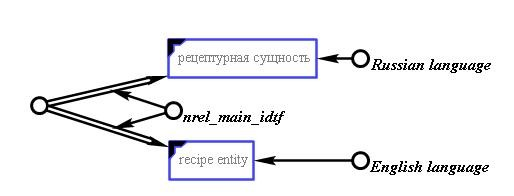
\includegraphics{images/chapter_3/рецептурная_сущность_главная_scg.jpg}
    \caption{Указание терминов ключевых элементов}
    \label{fig:recipe_entity_main_scg}
\end{figure}

\begin{figure}[H]
    \centering
    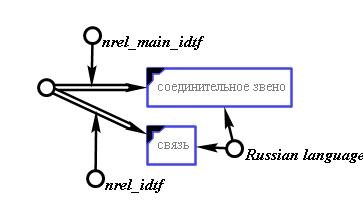
\includegraphics{images/chapter_3/рецептурная_сущность_синоним_scg.jpg}
    \caption{Указание синонимичных терминов}
    \label{fig:recipe_entity_synonym_scg}
\end{figure}

Другими ключевыми элементами в разделах документа являются:
\begin{itemize}
    \item обзорная модель (overview model),
    \item модель процессов (process model),
    \item модель технологического управления (procedural control model),
    \item модель рецептур (recipe model),
    \item физическая модель (physical model),
    \item модель оборудования (equipment model),
    \item модель деятельности управления (control activity model),
    \item планы рецептурного производства (batch schedule),
    \item история рецептурного производства (batch history) и отчёты (batch report),
    \item структуры обмена информацией (batch exchange table) и используемые типы данных,
    \item библиотеки технологических элементов (building block library and process element library):
          \begin{itemize}
              \item процессы (технологии),
              \item этапы процесса (процессы),
              \item операции процесса (производственные операции),
              \item действия процесса (фазы),
          \end{itemize}
    \item преобразования рецептур (transform components and transforming tasks),
    \item и другие.
\end{itemize}

Каждому выделенному ключевому элементу соответствует некоторая предметная область. Так, например, рецептурной сущности соответствует предметная область рецептов, а сущности оборудования соответствует предметная область оборудования.

На следующих этапах между представленными ключевыми элементами формируются структуры различного вида, в виде таксономий или реляционных структур, для этого используются обозначения соответствующих отношений, их связок и областей определения.

Предлагаемый подход позволяет интегрировать различные представления и модели, описывающие процессы и решения задач рецептурного производства, например, диаграммы переходов состояний в виде моделей ситуационного управления, указывающих режимы и описывающих состояния сущностей оборудования из модели оборудования и технологических элементов из модели процедурного управления, или процессная модель деятельности управления рецептурным производством.

На основе полученного в результате представления стандарта путём добавления агентов, способных решать задачи информационного поиска, можно строить интеллектуально справочные системы различного спектра, для этого необходимо добавить и использовать соответствующие уже разработанные агенты (например, поиска по образцу) в базу знаний. В этом случае системе управления знаниями предприятия, обладающей знаниями по стандарту ISA-88, можно задавать вопросы, в том числе связанные с поиском по образцу.

Рассмотрим некоторые аспекты построения онтологической модели предприятия рецептурного производства в соответствии со стандартом ISA-88.

\section{Модель оборудования предприятия}

В рамках перехода от традиционных АСУТП к интеллектуальным особый интерес представляет формализация документации предприятия, в частности технологических схем. Принципиальная простота взаимного перехода между технологическим чертежом и его семантическим представлением, дает возможность задавать вопросы, касающиеся элементов чертежа, инициировать команды, воздействующие на состояние соответствующего физического оборудования и отслеживать динамику состояния оборудования. Эта функциональность обеспечивается коллективом рецепторных и эффекторных агентов, работающих над семантическим представлением документации, хранящимся в общей семантической памяти. Это позволяет «оживить» техническую документацию предприятия, сделать ее многоцелевой. Таким образом, в зависимости от пользователя (оператор, мастер, начальник цеха) систем может давать нужные интеллектуальные ответы.

Модель оборудования строится на базе предметной области физических моделей рецептурных производств. Физическая модель (модель оборудования) в общем случае включает семь уровней:

\begin{itemize}
    \item блок управления (Control Module);
    \item агрегат (Equipment Module);
    \item установка (Unit);
    \item ячейка процесса (Process Cell);
    \item производственный участок (Area);
    \item производство (Site);
    \item предприятие (Enterprise).
\end{itemize}

Необходимо построить её структурную спецификацию на языке SCn.
